%Cooling Energy Savings Potential
For the cooling scenario, we calculate primarily the energy breakdown of the energy demands. The energy savings that can be achieved through improved set points is primarily from the variations of enthalpy differences, which represents the total energy that needs to be delivered by the HVAC systems. This can be further compared through the comparison of the differences between the cooling degree days calculated through the weather files. The total energy demand (sensible and latent) comapred with the sensible load only will not only provide us an estimation of the breakdown of the total energy demand, but also how these numbers vary by states and/or climate zones. 
	\begin{figure}[h!]
	\centering
	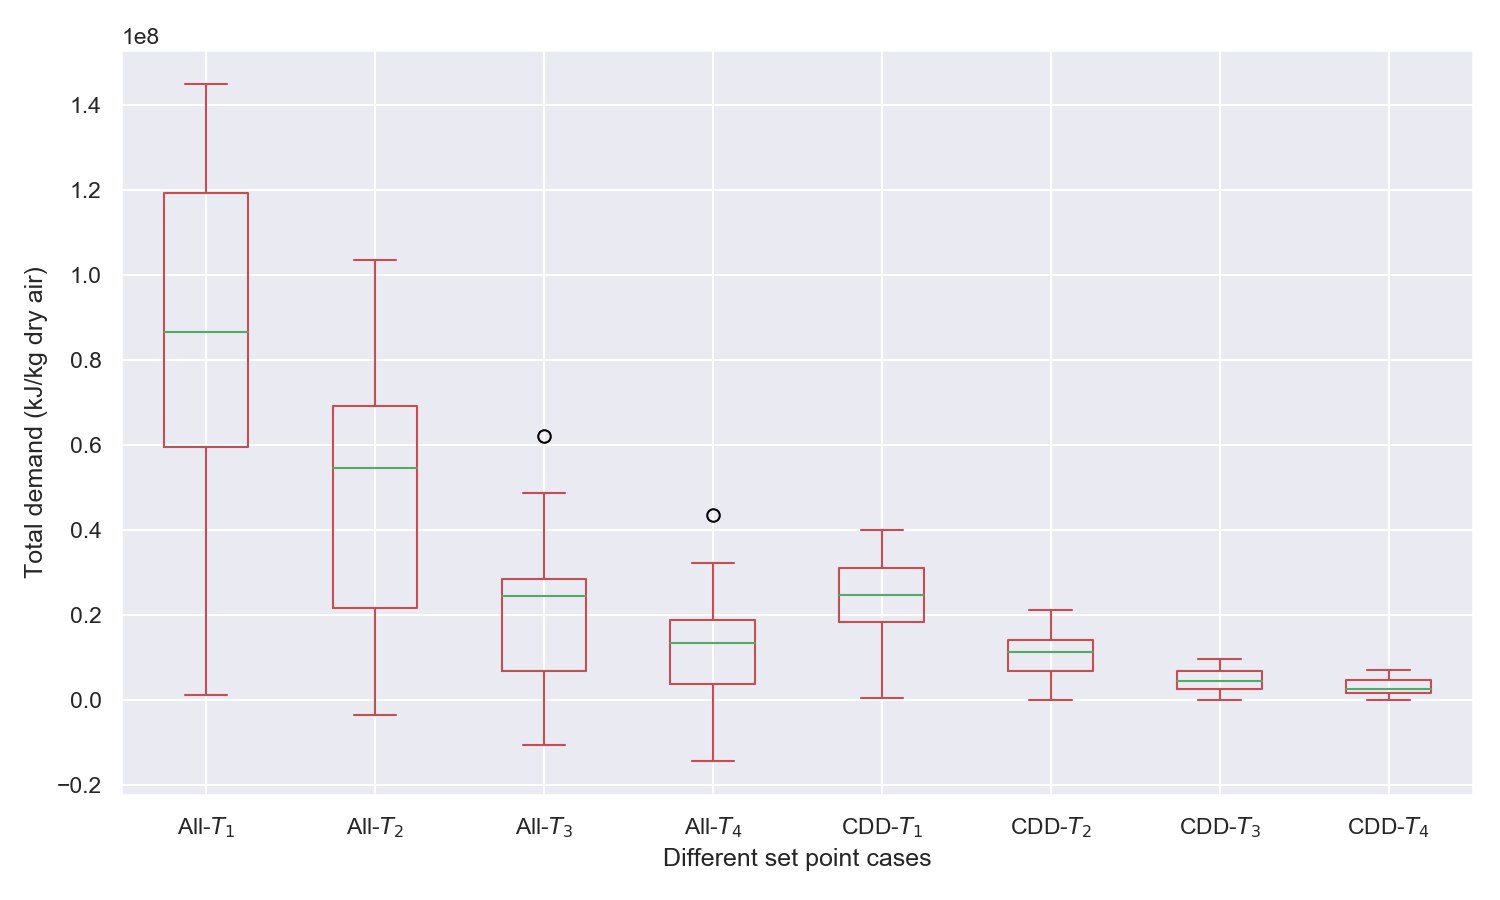
\includegraphics[width=0.8\textwidth]{coolheat.png}
	\caption{Box plot comparing the total energy demand from psychrometric analysis over dry-bulb only analysis}\label{fg:coolall}
	\end{figure}
The results we obtained for the by-state comparison are listed as the following box plot as indicated in Figure~\ref{fg:coolall}. The latent load that air-handling systems will need to address is much more significant than the differences we observed in the heating scenario, and when combined with teh sensible cooling load, exhibit apparent variations between different systems. The total energy requirement can be up to four times the sensible load when the set points are lower, and four times the sensible load when the set point is set higher. The order of magnitude of the overall enegy demand also changes significantly, with the total required energy of the air approximately 9 times of the one with the lowest set point. We must note that by assuming radiant systems, this energy requirement only covers the air instead of addressing the overall cooling load of the household. However, the energy that needs to be removed through dehumidification remains the same regardless, and needs to be properly characterized. We therefore expand this into a weather-station-specific study where we use the same weather data to analyze the station-specific latent loads under different set points. 

	\begin{figure}[h!]
	\centering
	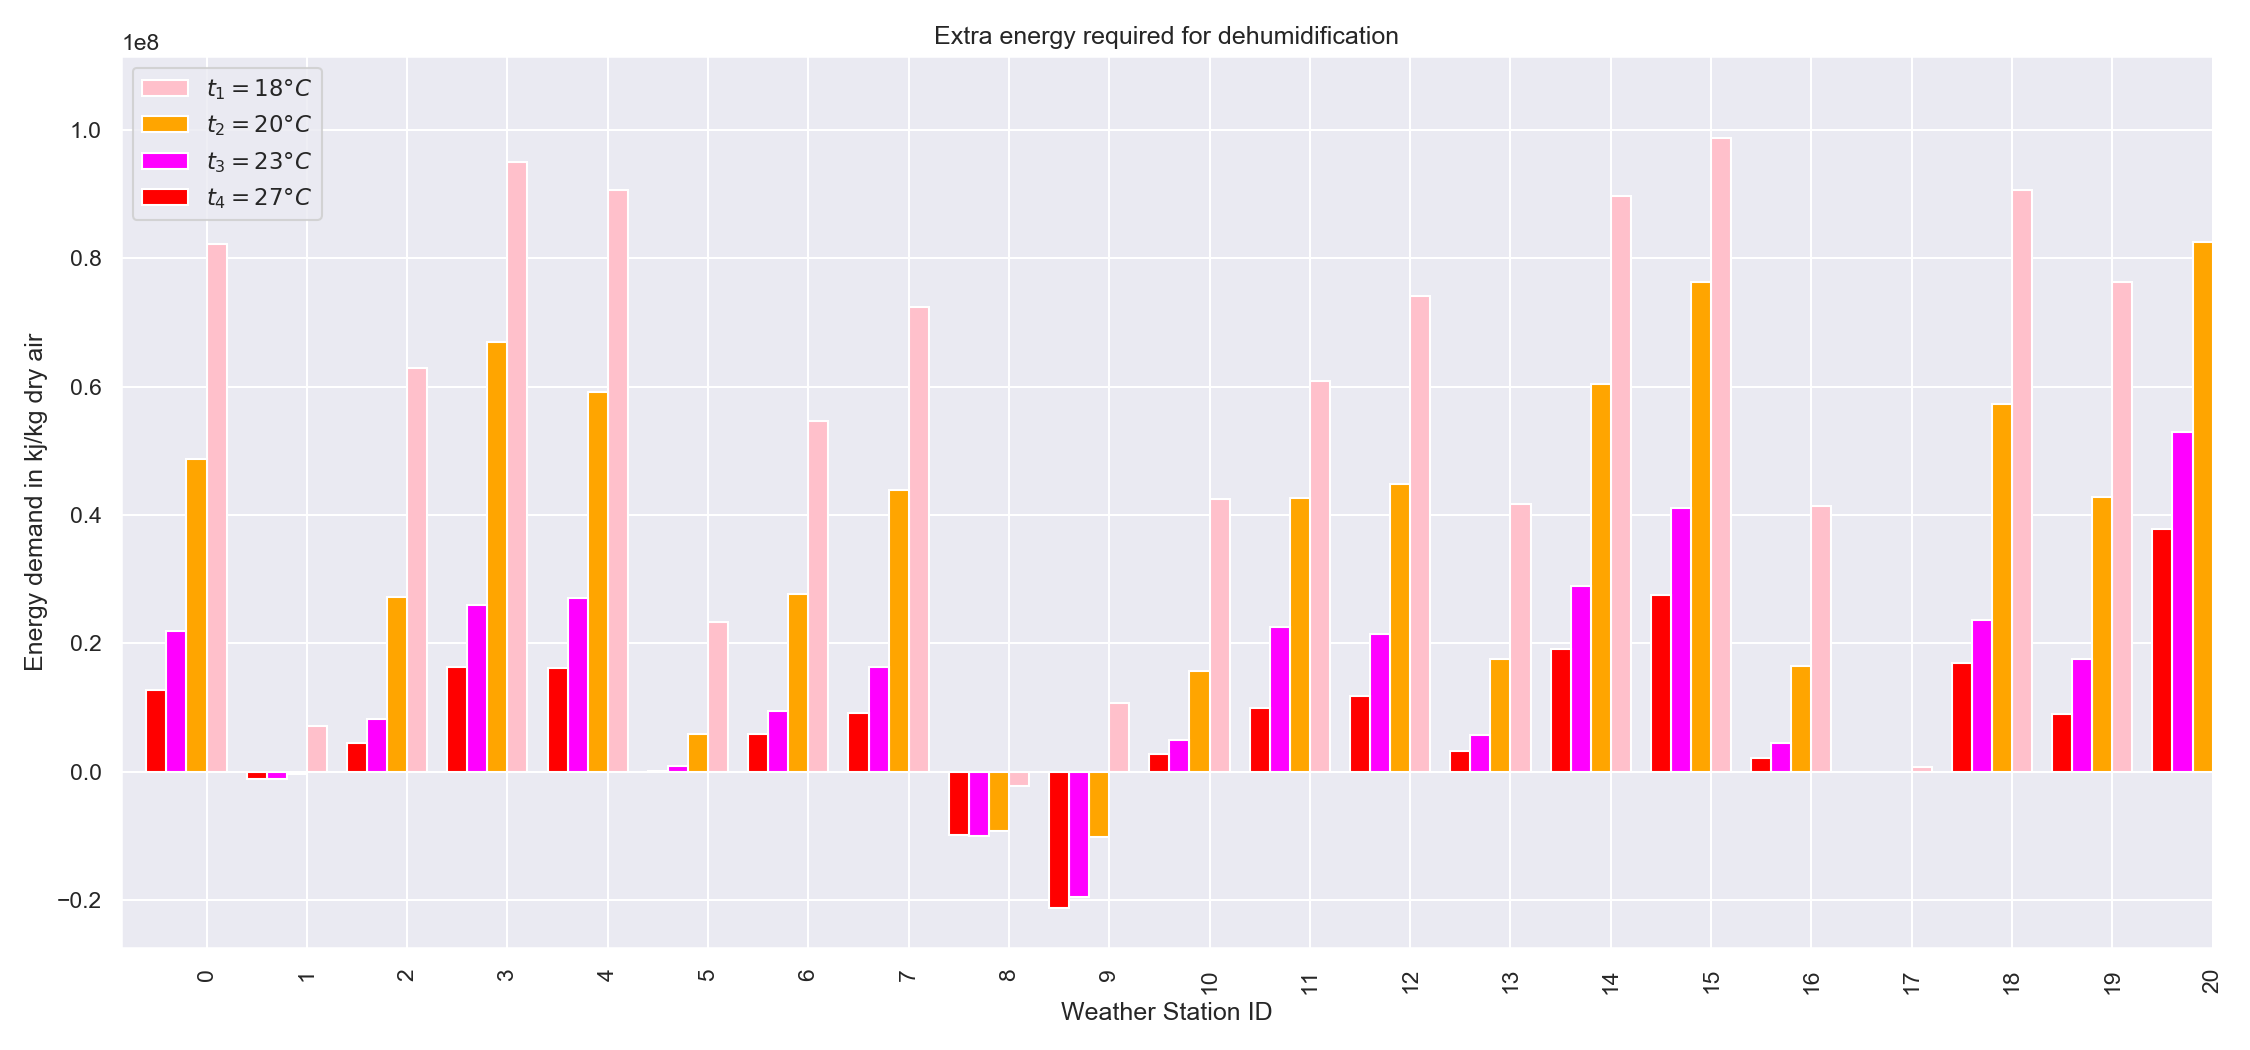
\includegraphics[width=0.8\textwidth]{coolsave.png}
	\caption{Box plot comparing the total energy demand from psychrometric analysis over dry-bulb only analysis}\label{fg:coolcities}
	\end{figure}

In Figure~\ref{fg:coolcities}, we compare the differences betweeen the energy required to condition different outdoor air condition when the outdoor air is processed to four different set points, i.e. $t_1$ through $t_4$ between $18 \degree C$ to $27 \degree C$. Out of all 21 weather stations, only 2 recorded summer (cooling) conditions that would not require additional dehumidification. 
Between different set points, the variations between the dehumidification demands are much higher. 
Compared to the heating scenario, the resulting temperatures are much higher. 

Also important to note is the `need for dehumidification' is not absolute, i.e. a 50\% relative humidity is the ideal condition, while in practice the relative humidity is not as tightly controlled. Existing methods of dehumidification (including reheat inside the air-handling units, solid and liquid desiccant or desiccant wheels) are predominantly designed to ensure the relative humidity stays below a more extreme RH level such that the growth of mold and bacteria can be prevented. For the purpose of this study, we selected an RH at 50\% for the sake of our argument. But in real building system operations, the cooling process indicated by the black arrrows in Figure~\ref{fg:cool} will likely only be determined by the system selected rather than the end state of the supplied (or room) air. 